\section{Blockchains}
Una blockchain è un registro (\textbf{ledger}) pubblico, condiviso e decentralizzato che memorizza la proprietà di beni digitali.\\
È quindi un registro in cui vengono memorizzate informazioni relative alla proprietà di qualcosa che può essere rappresentato tramite sequenze di bit. Vengono memorizzate anche le \textbf{transazioni}, ovvero i cambi di proprietà. Diciamo che un registro è pubblico dato che tutti possono vedere il registro, quindi chi possiede cosa e anche la storia della proprietà del bene.
Lo stesso registro è anche condiviso, quindi gestito da più persone, e decentralizzato in quanto non esiste un gruppo o una persona con poteri di amministratore, tutti sono allo stesso livello e possono fare le stesse cose. 

Il registro è organizzato in blocchi, dove abbiamo un primo blocco che dà il via alla blockchain (il \textbf{genesis block}) ed è seguito da una serie di blocchi che formano la catena blockchain.

I bocchi sono legati tra di loro mediante funzioni crittografiche particolari (\textbf{funzioni di hash crittografico}). Due blocchi sono collegati fra loro, se il valore di hash (impronta) di un blocco è contenuto all’interno del blocco successivo. Ciò rende altamente difficile alterare il contenuto di un blocco.
Un blocco contiene diverse transazioni (\textit{passaggi di proprietà}) che sono organizzate secondo una struttura dati particolare fatta in modo tale da rendere rapido e efficiente verificarne la validità. Del blocco corrente viene calcolato l’hash e inserito nel blocco successivo. Se si volesse modificare anche solo un bit del blocco, ci si troverebbe con un’impronta del blocco totalmente diversa, che non corrisponderebbe più a quella contenuta nel blocco ad esso collegato. È quindi sempre possibile (per tutti, in quanto è pubblica) verificare la validità della blockchain.\\
Modificare i dati cercando di fare in modo che il valore dell’impronta rimanga lo stesso è molto complicato.

Chi gestisce la blockchain è un insieme di utenti allo stesso livello. Gli utenti della blockchain sono nodi di una rete Peer-to-Peer (P2P). Sono delle reti dove ogni computer fa sia da client, quando necessita di informazioni da parte degli altri computer nella rete, sia da server, quando fornisce informazioni agli altri. \\
I nodi osservano le proposte di transazione che vengono fatte dagli utenti, che possono essere o membri stessi della rete P2P o altri utenti esterni, che decidono di non aiutare a gestire la blockchain ma di usarla. Questo può succedere perché la maggior parte delle persone infatti sono utenti che non vengono ingaggiati in un lavoro di gestione della blockchain. 
I nodi quindi verificano che le transazioni proposte siano valide, controllando per esempio che non avvenga il \textbf{double-spending}, ovvero non deve accadere la possibilità di cedere la proprietà di un bene contemporaneamente a due persone diverse.
I nodi devono poi eseguire un \textbf{protocollo di consenso}, per cui un certo numero di nodi della rete a un certo punto devono essere d’accordo sul fatto che le transazioni siano valide, che possano essere inserite in un blocco e che il blocco possa essere aggiunto in cima alla nostra blockchain. Questo passaggio serve perché i nodi possono essere chiunque, infatti un utente potrebbe scaricare la blockchain e fingere di essere un determinato utente cercando di truffare un altro utente. Non è quindi detto che siano tutti onesti. \\

Ad ogni aggiunta di un blocco alla catena, una copia della blockchain identica a tutte le altre viene memorizzata su ciascuno dei nodi della rete P2P (la nostra blockchain).
Fintanto che in una rete aperte (\textbf{permission less}, una rete dove può partecipare chiunque soltanto scaricando il software necessario per effettuare il mining) la maggior parte degli utenti di questi nodi è onesta si riesce a raggiungere un consenso valido. 

Succede il caso in cui ci sono due blocchi che vengono ritenuti entrambi validi e vengono quindi agganciati entrambi all’ultimo blocco della blockchain. Può succedere che in molte blockchain vengono aggiunti tutti e due e si inizia a lavorare su entrambi: il ramo che per primo riesce a proseguire in una catena più lunga diventa quello principale, sul quale si continuerà a lavorare (e quindi ad aggiungere blocchi), l’altro diventa un blocco \textbf{orfano}. \\
Le transazioni che si trovano sui blocchi dei rami (i rami di cui parliamo contengono i blocchi \textbf{orfano}), che vengono scartati diventano non più valide e vengono dimenticate; vanno quindi riconsiderate come transazioni proposte da inserire in uno dei prossimi nodi. Questo è un aspetto che se si presenta spesso rende la blockchain inefficiente.

Le transazioni sono \textbf{pseudo-anonimate} soprattutto se riguardano le criptovalute, in quanto si cerca di emulare le banconote reali per le quali non si sa per cosa sono state utilizzate in precedenza.

\begin{figure}[H]
    \centering
    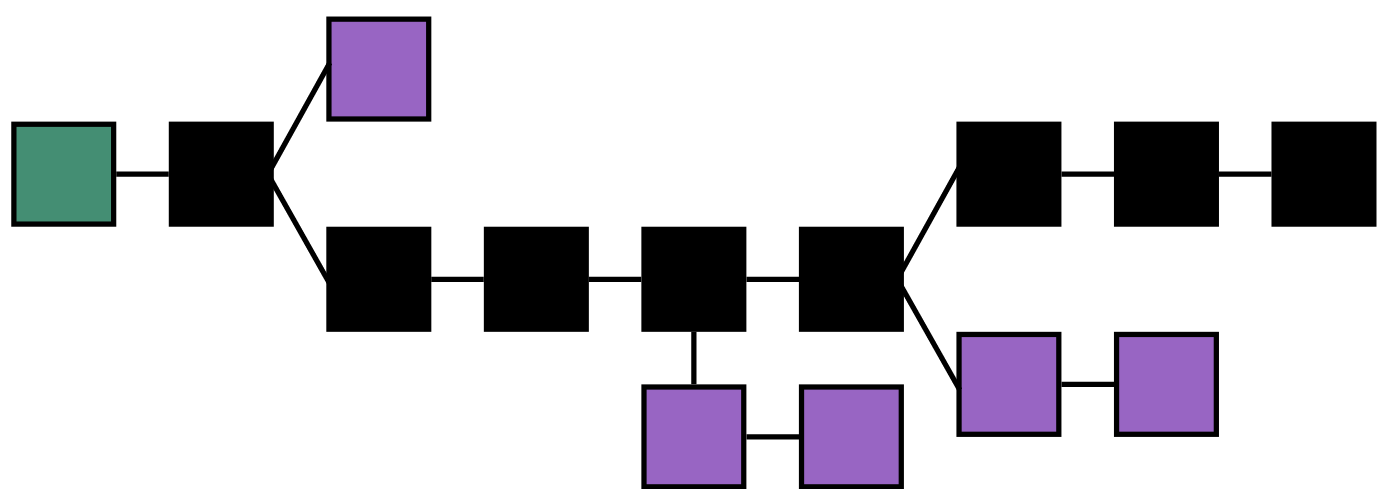
\includegraphics[scale = 0.25]{Immagini/c7f0503-reorg.png}
    \caption{Raffigurazione di una Blockchain}
    \label{fig:blockchain}
\end{figure}

Nella figura [\ref{fig:blockchain}] abbiamo in colore \textit{verde} i \textbf{genesis block}, in \textit{viola} i \textbf{orphan} e in \textit{nero} è rappresentata la blockchain composta dai nodi validi.

\subsection{Bitcoin}
Criptovaluta proposta nel 2008. nato anche per cercare di creare il sostituto digitale del denaro.
Il problema che potrebbe presentarsi riprende il \textbf{double spending}, infatti se una valuta digitale  ha un determinata firma hash collegata a un dispositivo, nulla mi vieta di copiare quella sequenza di bit e moltiplicare, virtualmente, la valuta di mio possesso e inviare la copia a una persona e mantenermi quelli iniziali io. Per evitare il problema del \textbf{double spending} si usa solitamente una \textbf{trusted third party}, per esempio la banca, che controlla e si segna i passaggi di proprietà.\\
La banca diventa però un collo di bottiglia e viene a sapere di tutti i trasferimenti di denaro, cosa che ai crittografi non piace. Nel 2008, l’idea è stata quindi quella di unire diversi protocolli crittografici e creare il bitcoin, dicendo che al posto della banca si usa un registro condiviso che tutti possono vedere dove si annotano le transazioni. \\

Le proprietà che vengono memorizzate sulla blockchain di bitcoin sono i bitcoin (BTC) o frazioni di essi (possono essere suddivisi in frazioni e sottofrazioni fino ad arrivare a $10^{-8} BTC$).\\

Le transazioni contengono diverse transazioni in ingresso, eventualmente altri campi particolare per generare nuovi bitcoin e alcuni script di transazione in output (script scritti in un linguaggio particolare). Se Alice vuole mandare a Bob un Bicoin usando il proprio client, a volta chiamato \textbf{wallet}, specifica la quantità che vuole mandare e un indirizzo. Ogni utente ha un indirizzo, che corrisponde a una lunga sequenza di numeri.  L’indirizzo si ottiene utilizzando la chiave pubblica (algoritmi a chiave pubblica). Attraverso un algoritmo opportuno, ogni utente si crea una chiave pubblica e una privata, rendendo pubblica la prima, che verrà utilizzata da chiunque voglia mandargli un messaggio.  \\
Per decifrare il messaggio l’utente utilizzerà la propria chiave privata. Dalla chiave pubblica di Bob a cui si applica una funzione di hash, Alice ottiene l’indirizzo di Bob. L’indirizzo è quindi una sorta di identità per l’utente, ma l’utente può generare tutte le copie di chiave pubblica e privata che vuole e quindi può utilizzare sempre indirizzi diversi. In seguito i bitcoin ottenuti su diversi indirizzi si possono poi combinare. \\ Ma come fa Alice a dimostrare che Lei è la proprietaria di quel Bitcoin e che quindi ha la possibilità di mandarlo a Bob? Questa transazione la firma con la firma digitale e invia la transazione a Bob. \\
La firma digitale viene applicata utilizzando la chiave segreta del mittente (Alice), al fine di dimostrare la propria identità.
I nodi P2P verificano quindi che la firma del mittente sia valida e che la somma di bitcoin mandata non sia già stata inviata ad altri, quindi che la transazione sia valida in caso positivo viene aggiunta alla blockchain. \\
Il fatto di possedere un Bitcoin è indicato dal fatto che sia possibile iniziare una transazione per mandarlo a qualcun altro e quindi che si possieda una chiave segreta, che dobbiamo salvarci essendo molto importante. 
Nelle blockchain non si registra il numero di Bitcoin posseduti dagli utenti ma la storia dei Bitcoin (i loro passaggi di proprietà) e quindi le transazioni.

\subsubsection{Miners}
I miners sono  i membri della rete P2P. \\
Esiste un pool di transazioni che vengono proposte dai vari client (\textbf{wallet}) e i miners osservano le transazioni, ne scelgono un migliaio che vengono validate e cercano di formare il nuovo blocco (circa uno ogni 10 minuti). Dopo aver validato le transazioni eseguono le operazioni computazionali collegate al cosiddetto \textbf{proof-of-work}. I miners devono dimostrare di avere effettuato una certa computazione per aver diritto di aggiungere il prossimo blocco alla catena. La computazione da fare e quindi la creazione del blocco diventa sempre più difficile. \\

Le funzioni di hash sono funzioni crittografiche che prendono in input una sequenza di bit (in teoria arbitrariamente lunga, in pratica il limite per la lunghezza è molto alto e non lo si raggiunge mai) e produce una sequenza di poche centinaia di bit (che vorrebbe essere unica). Dato che il dominio della funzione di hash è molto più grande del codominio può capire che l’hash di due file diversi produca in output la stessa sequenza di bi, in questo caso si ha una \textbf{collisione}. \\

Le collisioni esistono ma sono molto rare, e quindi si può pensare che ogni impronta (\textbf{valore della funzione id hash}) sia associata univocamente al file da cui è stata calcolata. Più difficile ancora è, dato un input con una certa impronta, trovare un altro input che abbia la medesima impronta. \\
Data un’impronta, è estremamente difficile trovare un input che produce una determinata impronta (la funzione di hash è \textbf{one-way}, ovvero facile da calcolare ma difficile da invertire). \\ 
Anche se si cambia un solo bit dell’input si ottiene un output completamente diverso, non si possono quindi cercare correlazioni statistiche o cercare di capire quale sia la regola con cui vengono calcolate. \\

Nella textbf{proof-of-work} si deve dimostrare di aver svolto una certa quantità di lavoro. Viene preso il dato di cui si deve calcolare l’hash e gli si aggiunge una certa quantità casuale, chiamata \textbf{nonce}, e si calcola l’hash di questa concatenazione.In seguito vado a vedere se il risultato ha un certo numero prefissato di bit più significativi uguali a 0, così facendo si riduce il codominio, e quindi il numero possibile di output validi in quanto devono iniziare con un certo numero di 0. Se si aumenta il numero di 0, si rende meno probabile il fatto che sparando a caso un nonce si ottenga un risultato valido. Ciò rende più difficile creare le impronte e quindi i blocchi. Al contrario se si diminuisce il numero di 0 richiesti, lo si rende più facile. \\
Quando finalmente il \textbf{miner} riesce a creare il blocco, questo viene mandato nella rete P2P e gli altri miners ne controllano la validità. Se ne riscontrano la validità il blocco viene inserito in cima ad ogni copia della blockchain.

Mentre un miner sta lavorando a un blocco B e qualcuno ne propone prima un altro B’ che viene aggiunto, il miner, per poter ancora proporre B, deve scartare le transazioni di B che già compaiono in B’ e aggiungere l’hash di B’ nell’intestazione di B. L’unico momento in cui si possono creare dei nuovi bitcoin è durante la creazione di un nuovo blocco: chi riesce ad aggiungere un nuovo blocco alla catena ha dei nuovi bitcoin. I bitcoin creabili in un blocco sono in numero limitato (se ne possono costruire al massimo 21 milioni). Il mercato delle criptovalute è un mercato non regolamentato soggetto a manipolazione.

Un problema del decentramento è l'\textbf{Attacco del 51$\%$}, infatti se si controlla, o si possiede, il 51$\%$ della potenza di calcolo di tutti i miners, si ha sempre il controllo di quale blocco viene aggiunto. Un problema ulteriore è il \textbf{problema dello spreco di energia}, si è verifiato che un tipo di confronto tutti contro tutti (tra miner) è molto inefficiente, la rete P2P che gestisce la blockchain di bitcoin consuma più dell’Argentina. Si cercano quindi algoritmi per esempio per la creazione del consenso diversi dalla \textbf{proof-of-work}, un algoritmo potrebbe essere la \textbf{proof-of-stake}.\\

Lo stake è la quantità di soldi. Non tutti fanno il mining, ma solo un sottoinsieme di nodi viene scelto per validare le transazioni. Il sottoinsieme viene scelto in maniera direttamente proporzionale alla quantità di soldi che si è deciso di bloccare (di rendere disponibile agli altri) su un conto speciale. Chi mette più soldi ha più probabilità di essere scelto. \\

Il fatto che ci sia un numero massimo di bitcoin creabili e che creali diventi sempre più difficili ha fatto paragonare i bitcoin all’oro (oro digitale).

\subsubsection{Altro esempio}
Prendiamo in considerazione il caso in cui Alice vuole dare una porzione dei bitcoin a Bob.
Se Alice possiede 10 bitcoin e ne vuole dare 1 a Bob. Allora Alice deve creare 2 transazioni una in cui a partire dall’input di 10 BTC  produce un output verso Bob e un’altra in cui contemporaneamente a partire dall’input 9 produce un output a se stessa. In sostanza Alice deve effettuare due transazioni una in cui fornisce i suoi bitcoin a Bob e una con cui si dà il resto. La somma totale data in input a Bob non dev’essere minore della somma in output (verso Alice). La somma in input può infatti essere maggiore perché la differenza tra i bitcoin totali mandati e quelli che si vogliono fare avere a Bob costituirebbe una \textbf{fees}, un compenso che viene dato al miner. \\ I miner selezioneranno per prime le transazioni del pool che hanno le \textbf{fees} più alte. Le transazioni con \textbf{fees=0}, difficilmente vengono considerate e perciò vengono dette \textbf{transazioni zombie}. \\

Per essere ragionevolmente sicuri che una transazione sia andata a buon fine si devono aspettare circa 6 blocchi (un’ora), quindi non è possibile utilizzare i bitcoin per piccole e rapide transazioni (comprare il giornale).

\subsection{Ethereum}
Un'altra tipologia di block chain in cui si pone l’attenzione non sulle transazioni, ma sulle computazioni. Non vengono memorizzate le transazioni come bitcoin, ma all’interno di Ethereum ogni utente ha un account nel quale ha una certa quantità di criptovaluta (\textbf{ether ETH}). Le transazioni avvengono esattamente come per i bitcoin.\\ 
In Ethereum c’è la possibilità di scrivere gli \textbf{smart contract}, sono il corrispettivo dei contratti tra persone (si dà in uso un bene e si chiede in cambio un compenso mensile). Gli smart contract sono scritti con il linguaggio di programmazione \textbf{Solidity}.

I contratti vengono compilati in un bytecode (linguaggio macchina della Etherum VM) e quest’ultimo viene memorizzato in tutte le copie della blockchain di Ethereum. Un client può fare una transazione in cui o trasferisce soldi o chiama una funzione all’interno di un contratto. Durante le transazioni uno dei miner raccoglie la transazione che esegue un contratto e lo esegue sulla sua macchina. Ogni esecuzione di ogni singola operazione del bytecode costa una certa quantità di \textbf{gas}, ovvero una certa quantità di soldi che si è disposti a spendere per l’esecuzione del contratto (se ne dovessero avanzare, la parte in più viene restituita). Nel caso in cui non si abbiano abbastanza soldi per eseguire un contratto, viene sollevata un’eccezione \textbf{Out of gas}: i soldi spesi vengono persi e il contratto non va a buon fine perché dà errore.
Gli smart contract sono codice lato server di cui chiunque può vedere il bytecode. I tempi di esecuzione sono lenti, parlando di un ambito molto delicato come il denaro. 

\subsubsection{Tipologie di Blockchain}
Ci sono diversi tipi di blockchain.
\begin{itemize}
    \item Permissionless: dove chiunque può scaricarsi il software e diventare miner, non ha bisogno di permessi particolari.
    \item Permissioned (publica e privata): dove i nodi della rete P2P (che sono quelli che possono scrivere, avviare le transazioni) si conoscono uno con l’altro ma non si fidano, motivo per cui scrivono pubblicamente sulla blockchain(public blockchain). 
    I miners sono potenzialmente in conflitto fra loro: ci guadagnano dalle perdite degli altri.(private blockchain)
\end{itemize}
Inoltre si può verificare la necessità di utilizzo di una blockchain e del tipo necessario. Come possiamo notare dalla figura [\ref{fig:do_i_need}]. 

\begin{figure}[H]
    \centering
    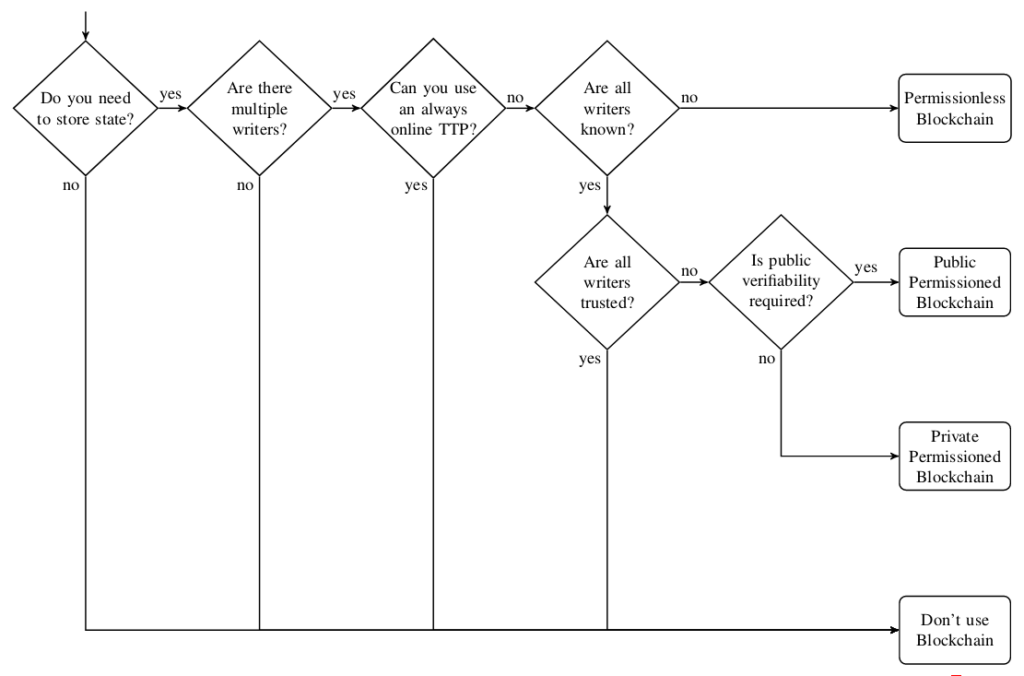
\includegraphics[scale = 0.3]{Immagini/blockchain-it-1024x676.png}
    \caption{Ho veramente bisogno di una blockchain?}
    \label{fig:do_i_need}
\end{figure}
